\section{8086, 80186,80286,8038 (16-bit) memory interface}
\begin{itemize}
  \item \textbf{80286/80386}: 24-bit address bus. $\overline{MRDC}$ and $\overline{MWTC}$ instead of $\overline{RD}$ and $\overline{WR}$.
  \item These $\mu P$s must be able to write data to any 16-bit or 8-bit location. Therefore, the 16-bit data bus must be divided into two separate sections (banks), which are 8-bit wide.
\end{itemize}

\begin{figure}[h!]
  \centering
    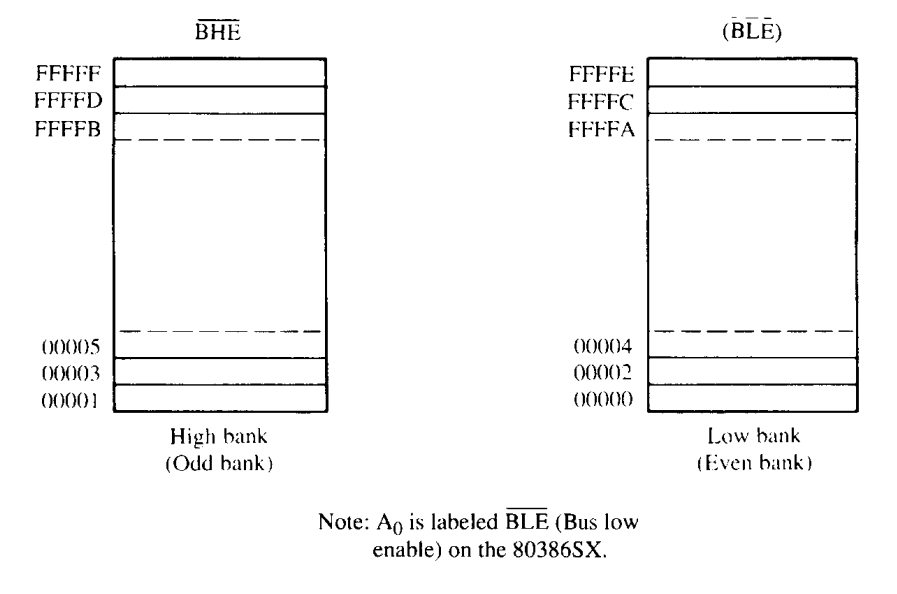
\includegraphics[width=0.9\textwidth]{./figures/Bank_Enable.png}
    \caption{The high (odd) and low (even) 8-bit memory banks of the 8086/80286/80386SX microprocessors.}
    \label{fig:BHE}
\end{figure}
\newpage
\begin{figure}[h!]
  \centering
    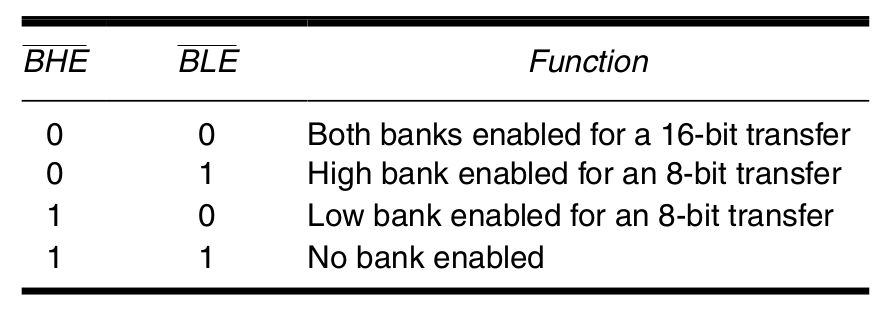
\includegraphics[width=0.9\textwidth]{./figures/Bank_Table.png}
    \caption{Memory bank selection using $\overline{BHE}$ and $\overline{BLE}$ ($A_0$).}
    \label{fig:BHE_Table}
\end{figure}

Bank selection is accomplished in two ways:
\begin{enumerate}
  \item A separate write signal is developed to select a write to each bank (least costly)
  \item Separate decoders are used for each bank
\end{enumerate}


\begin{figure}[h!]
  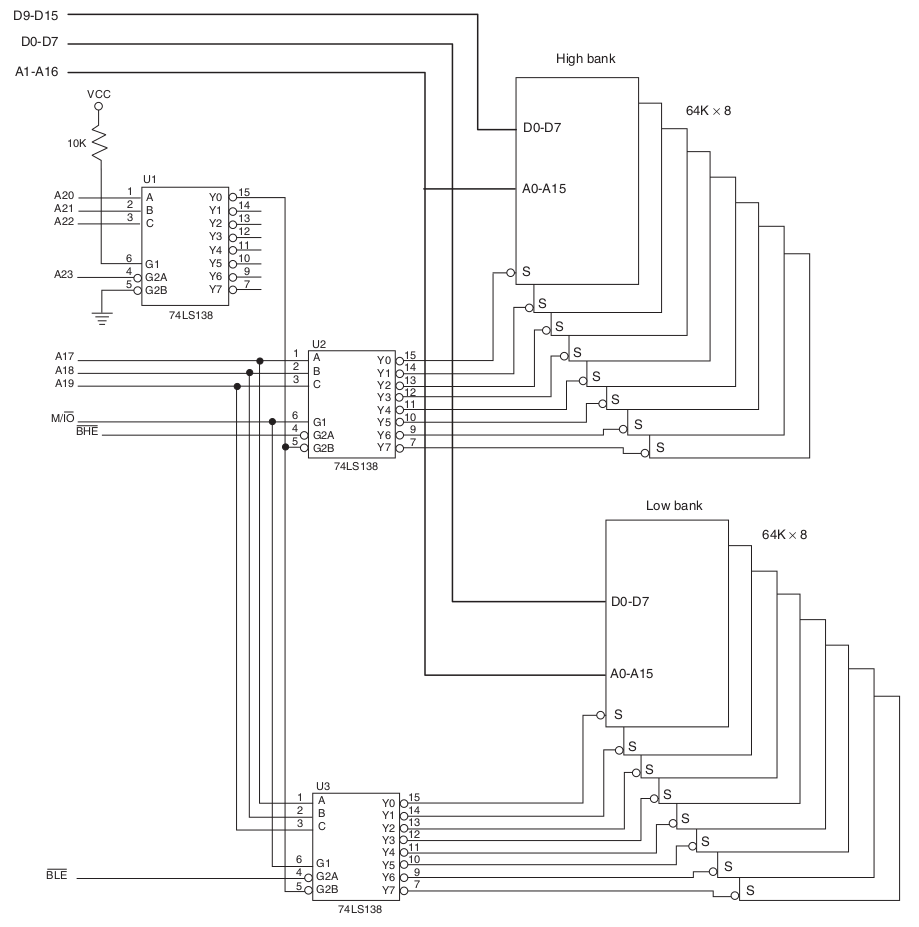
\includegraphics[width = 0.9\textwidth]{./figures/Bank_Separate.png}
  \caption{Separate bank decoders.}
  \label{}
\end{figure}
\begin{itemize}
  \item Two 74LS138 decoders are used to select 64K RAM for 80386 $\mu P$ (24-bit address)
  \item An enable pin (G2A) of U3[First 74LS138] is enabled by $\overline{BHE}$ and of U2[Second 74LS138] is enabled by $\overline{BLE}~(A_0)$.
  \item U3 controls enabling the high bank, and U2 controls enabling the low bank.
  \item Decoded memory location range is \textbf{000000H-0FFFFFH}(1M).
  \item $A_0$ (or $\overline{BLE}$) is \textbf{not} connected to the memory to ensure having separate memory address (odd  or even) in separate banks. If it would be connected to the memory address pin, the half of the memory will be wasted.
  \newline [$A_0$ is \textbf{NOT} even a pin in 80386 $\mu P$]
\end{itemize}

\newpage
\section{8086 (16-bit) memory interface}
\textbf{Separate bank write strobes for memory}: $\overline{WR}$ combines with $A_0$ for low bank selection ($\overline{LWR}$), and $\overline{BHE}$ for high bank selection ($\overline{HWR}$)
\newline
For 80286 and 80386: $\overline{MWTC}$ is used instead of $\overline{WR}$
\begin{figure}[h!]
  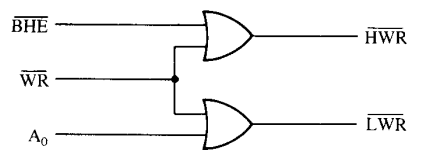
\includegraphics[width = 0.6\textwidth]{./figures/Bank_8086.png}
  \caption{The memory bank write selection input signals: $\overline{HWR}$ (high bank write) and $\overline{LWR}$ (low bank write).}
  \label{}
\end{figure}
\newline
\textbf{Why not also generate read strobe for each memory bank ?}\newline
\begin{itemize}
  \item It is usually unnecessary as 086, 80286, 80386 $\mu P$s read only the byte of data they need at any given time ignoring the other parts without causing any problem.
  \item \textbf{Example}: 16-bit memory stored at locations 060000H-06FFFFH for 80286 or 80386 $\mu P$ using PAL
  \item PAL logics:
  \begin{enumerate}
    \item $\overline{CS} = \overline{A23} \cdot \overline{A22} \cdot \overline{A21} \cdot \overline{A20} \cdot \overline{A19} \cdot \overline{A18} \cdot \overline{A17} \cdot \overline{A16}$
    \item $\overline{LWR} = \overline{MWTC} \cdot \overline{A_0}$
    \item $\overline{HWR} = \overline{MWTC} \cdot \overline{BHE}$
  \end{enumerate}
\end{itemize}
\textbf{Extend this concept of separate banking for all subsequent design (32, 64, ... bits) *** SELF STUDY ***}
\newpage

\begin{figure}[h!]
  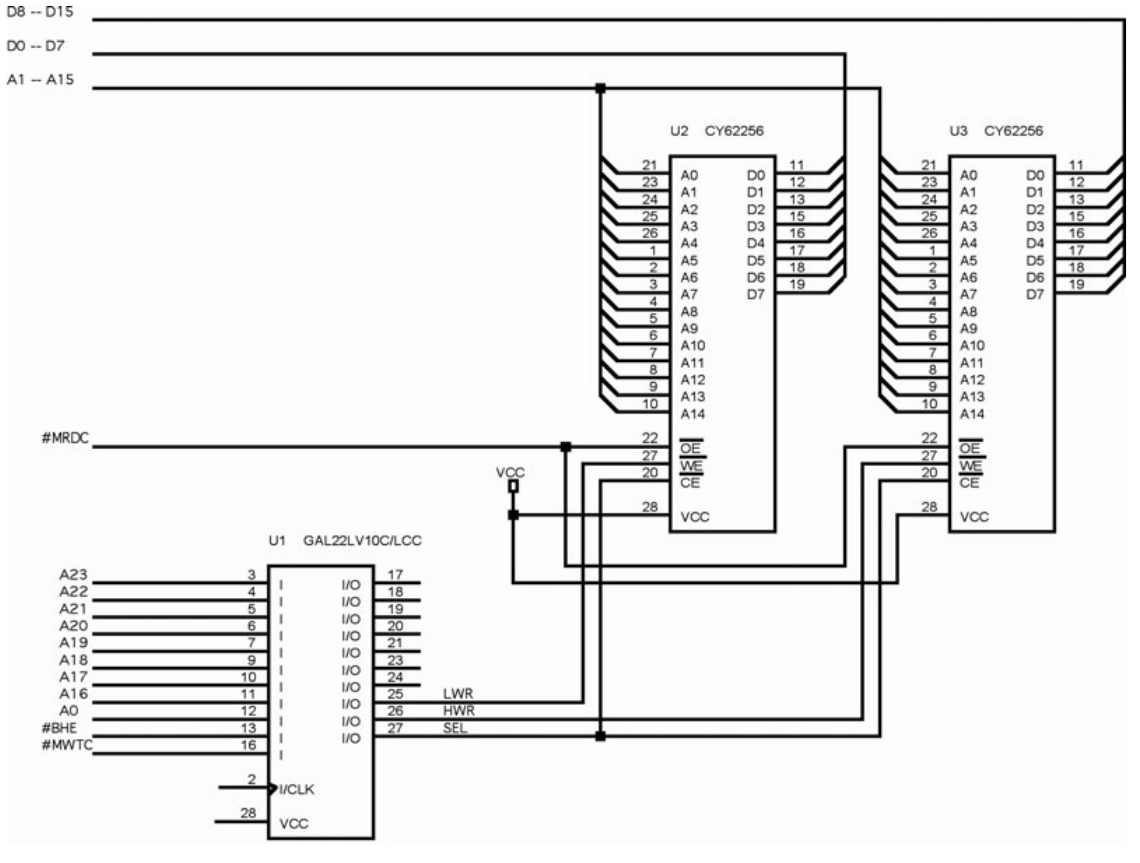
\includegraphics[width = 1.0\textwidth]{./figures/Separate_Bank.png}
  \caption{A 16-bit-wide memory interfaced at memory locations 06000H–06FFFH.}
  \label{}
\end{figure}

\textbf{Example}: A memory system for 8086 containing 64K byte EPROM and 128K byte SRAM.
\begin{itemize}
  \item $\overline{RD}$ is connected to all $\overline{OE}$ inputs (enabling all 16-bits while reading).
  \item $\overline{LWR}$ and $\overline{HWR}$ are connected to different banks of RAM. Here, both $\overline{LWR}$ and $\overline{HWR}$ go low. For 8-bit eriting, either of them goes low. Such writing is \textbf{not} needed for EPROM
  \item A 74LS139 (dual 2-to-4 decoder) is used to select EPROM with one half and RAM with the other half. It decodes memory as 1-bit wide ( not 8-bit).
  \item EPROM's decoder signal is sent to 8086 wait state generator.
\end{itemize}

\begin{figure}[h!]
  \centering
  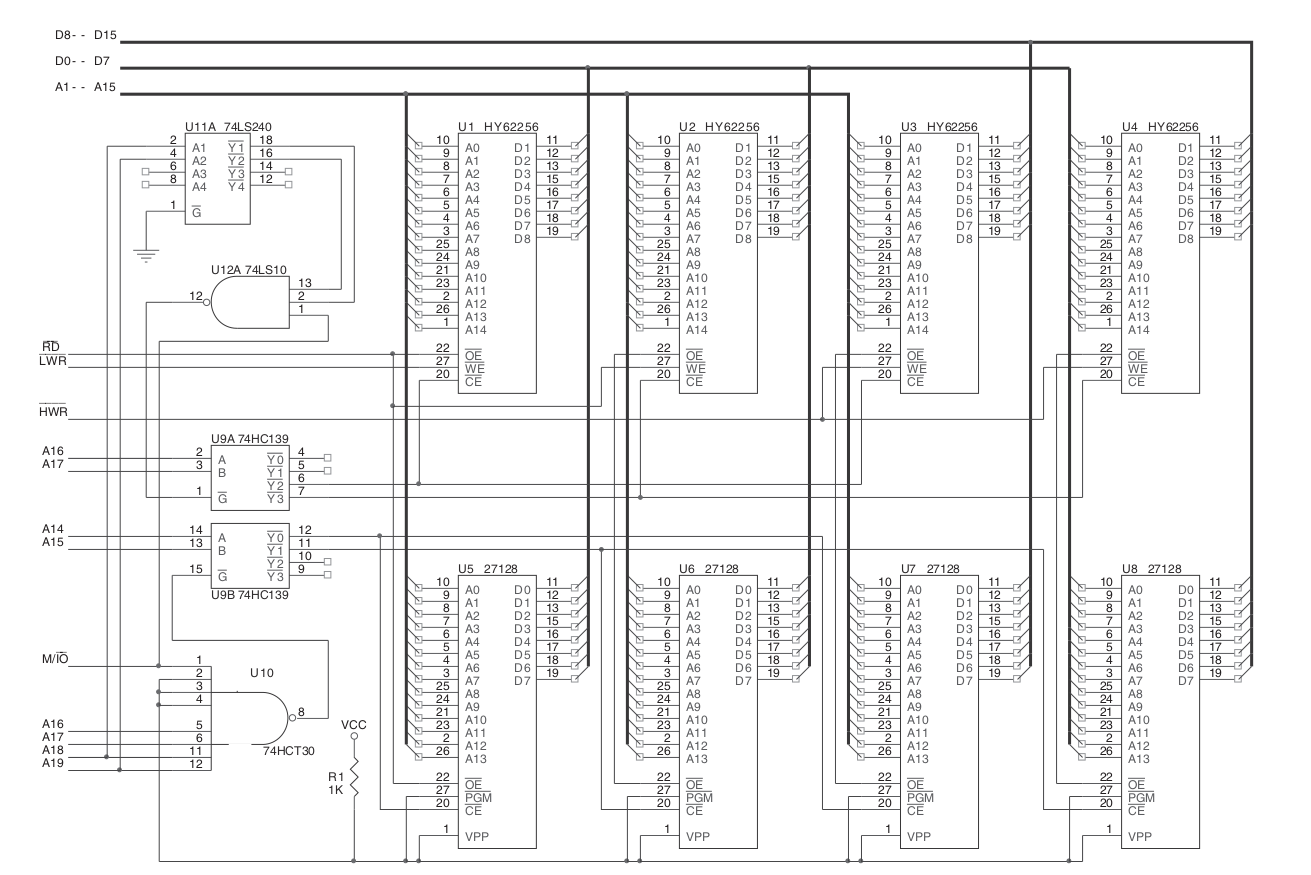
\includegraphics[width = 1.2\textwidth]{./figures/Memory_System.png}
  \caption{A memory system for the 8086 that contains a 64K-byte EPROM and a 128K-byte SRAM.}
  \label{}
\end{figure}
